\chapter{Introduction}

Neutrinos are elusive fundamental particles of great importance in the continuing study of particle physics.  Though extremely difficult to study, with tiny yet non-zero masses, no electric charge, and low interaction cross-sections, neutrinos have provided great insight into nuclear physics, geophysics, and astrophysics, and may provide the key to understanding the matter/anti-matter asymmetry of the universe.  Neutrinos were first predicted by W. Pauli in 1930.  He proposed the existence of a neutral, unobserved particle to explain the apparent violation of energy conservation in beta decay \cite{betaspectrum}. He admitted that neutrinos (then deemed ``neutrons'' -- what we now know as neutrons had not been discovered yet either) should be difficult to observe experimentally, but also that it seemed unlikely that they would never have been noticed before.  As it turns out, they are much more difficult to observe than he predicted.  Their probabilities for interaction are extremely small.

A theory formulated in 1933 by E. Fermi for beta decay \cite{FermiBetaDecay}, including the neutrino, was the beginning of weak interaction theory.  Eventually, progress led to a unified treatment of electromagnetic, weak and strong forces and the development of the very successful Standard Model (SM) of particle physics.  In the SM, neutrinos are massless.  The discovery of non-zero neutrino mass via neutrino oscillations in the late 1990s \cite{SuperK} shows that there is more new physics to be discovered beyond the SM, and presents a path to follow.

The See-Saw Mechanism is a theory which explains the extreme lightness of neutrinos compared to other particles, while also predicting very heavy neutrino partners.  The existence of heavy neutrinos in the high-energy environment of the early universe, coupled with the possibility of the violation of CP conservation in decays of these heavy neutrinos, could explain why the universe became dominated by matter \cite{SeeSaw}.

If neutrinos are Majorana particles rather than Dirac particles, the process of neutrinoless double beta decay ($0\nu\beta\beta$) is allowed if the neutrino mass is non-zero.  Observation of $0\nu\beta\beta$ would simultaneously demonstrate that neutrinos are Majorana particles, as well as aid in determining the absolute mass itself \cite{effectiveMass}.  This chapter outlines the current theory for neutrinos, and then describes the $0\nu\beta\beta$ experiments EXO-200 and nEXO, in order to motivate barium tagging for nEXO.

\section{Neutrinos}

Neutrinos are chargeless leptons which only interact via the weak force (and gravity).  There are three known ``flavors'' of neutrinos, $\nu_{e}$, $\nu_{\mu}$, and $\nu_{\tau}$, each corresponding to one of the three known leptons.  These are the eigenstates in the basis of the weak force, so they are the states in which a neutrino will interact via the weak force.

\subsection{Neutrino Oscillation and Mass}

If neutrinos have a mass basis which is different from the flavor basis, the phenomenon of flavor oscillation may occur.  Neutrinos, which are produced as pure flavor states, will exhibit a time-dependent oscillation in the probability of measuring the other flavors as well.  

The very small mass of a neutrino relative to its momentum lets one write the relativistic Hamiltonian in terms of mass squared differences $\Delta m_{ij}^{2} = m_{i}^{2} - m_{j}^{2}$, where $i$,$j$ = 1,2,3, referring to the three mass states.  The mixing between the 3-vector mass and flavor bases is defined by a rotation in terms of three mixing angles, $\theta_{12}$, $\theta_{23}$, and $\theta_{13}$.  Transformation between the flavor and mass bases is done with the following unitary matrix, called the Pontecorvo--Maki-–Nakagawa–-Sakata (PMNS) matrix \cite{ReviewNuMass}:

%The mass basis is really the energy basis with the small mass approximation, along with dropping some constant terms in the Hamiltonian (which do not affect time evolution).

\begin{equation}
\begin{aligned}
U &= \begin{pmatrix}
1 & 0 & 0 \\
0 & c_{23} & s_{23} \\
0 & -s_{23} & c_{23} \end{pmatrix}
\begin{pmatrix}
c_{13} & 0 & s_{13} e^{-i \delta} \\
0 & 1 & 0 \\
-s_{13} e^{i \delta} & 0 & c_{13} \end{pmatrix}
\begin{pmatrix}
c_{12} & s_{12} & 0 \\
-s_{12} & c_{12} & 0 \\
0 & 0 & 1 \end{pmatrix}
\begin{pmatrix}
1 & 0 & 0 \\
0 & e^{i \alpha_{1}/2} & 0 \\
0 & 0 & e^{i \alpha_{2}/2} \end{pmatrix} \\
& = \begin{pmatrix}
c_{12} c_{13} & s_{12} c_{13} & s_{13} e^{-i \delta} \\
-s_{12} c_{23} - c_{12} s_{23} s_{13} e^{i \delta} & c_{12} c_{23} - s_{12} s_{23} s_{13} e^{i \delta} & s_{23} c_{13} \\
s_{12} s_{23} - c_{12} c_{23} s_{13} e^{i \delta} & -c_{12} s_{23} - s_{12} c_{23} s_{13} e^{i \delta} & c_{23} c_{13} \end{pmatrix}
\begin{pmatrix}
1 & 0 & 0 \\
0 & e^{i \alpha_{1}/2} & 0 \\
0 & 0 & e^{i \alpha_{2}/2} \end{pmatrix}
\end{aligned}
\label{eqn:umatrix}
\end{equation}

\noindent
where $c_{ij} = \cos \theta_{ij}$, $s_{ij} = \sin \theta_{ij}$.  $\delta$  and $\alpha_{i}$ are Dirac and Majorana CP-violating phases, respectively.  Transformation between bases is done by Eq. \ref{eqn:nuTransform}:

\begin{equation}
\begin{aligned}
\ket{\nu_{\alpha}} &= \sum\limits_{i} U^{*}_{\alpha i} \ket{\nu_{i}},\\
\ket{\nu_{i}} &= \sum\limits_{\alpha} U_{\alpha i} \ket{\nu_{\alpha}}.
\end{aligned}
\label{eqn:nuTransform}
\end{equation}

A two-neutrino approximation demonstrates how this results in neutrino oscillation.  In this case, there is only one mixing angle $\theta$ and one mass squared difference $\Delta$, and the Hamiltonian $H$ and mixing matrix $U$ are as follows:

\begin{equation}
\begin{aligned}
H &= \frac{1}{4 E} \begin{pmatrix}
-\Delta & 0 \\
0 & \Delta
\end{pmatrix} \\
U &= \begin{pmatrix}
\cos \theta & \sin \theta \\
-sin \theta & \cos \theta
\end{pmatrix}.
\end{aligned}
\end{equation}

\noindent
Applying time evolution to a pure electron neutrino state (where the two neutrino flavors here are $\nu_{e}$ and $\nu_{\mu}$) then leads to the following time-dependent state:

\begin{equation}
\begin{aligned}
\ket{\nu(t)} = (e^{i t \Delta / 4 E} \cos^{2} \theta + e^{-i t \Delta / 4 E} \sin^{2} \theta) &\ket{\nu_{e}} \\ + \cos \theta \sin \theta (-e^{i t \Delta / 4 E} + e^{-i t \Delta / 4 E}) &\ket{\nu_{\mu}}
\end{aligned}
\label{eqn:oscilprob}
\end{equation}

\noindent
where $E$ is the neutrino energy.  Note that if $\theta$ is zero, the case where the mass basis is the same as the flavor basis, the state remains pure $\ket{\nu_{e}}$.  The same is true if $\Delta$ is zero.  Thus, the discovery of neutrino oscillation was the first (and only, so far) demonstration that neutrinos have a non-zero mass.
%\emph{\color{gray}(particularly a non-zero mass squared difference)}.

Studying oscillations of neutrinos from different kinds of sources, with different energies and path lengths, can isolate sensitivities to the different mixing angles and mass squared differences.  For example, the study of solar neutrinos (neutrinos emanating from nuclear fusion reactions in the core of the sun) provides sensitivity to $\theta_{12}$ and $\Delta m_{21}^{2}$.  The oscillation parameters so far measured are shown in Table  \ref{table:nu_osc_vals}.

\begin{table}[!htbp]
\caption{Best-fit values for neutrino oscillation parameters, from a global fit to oscillation experiment data.   Parameters which depend on the mass hierarchy have separate values for NH (IH).  The atmospheric parameter $\Delta m^{2}$ is defined as $\Delta m^{2} = \Delta m_{31}^{2} - \Delta m_{21}^{2}/2 > 0 (\Delta m^{2} = \Delta m_{32}^{2} + \Delta m_{21}^{2}/2 < 0)$. \cite{ReviewNuMass}} %not sure what [Small Table], between \caption and {}, w/ no spaces, does
\label{table:nu_osc_vals}
\begin{tabular}{c|l}
Parameter & Measurement ($\pm 1 \sigma$) \\
\hline
$\Delta m_{21}^{2}$ & 7.54$^{+0.26}_{-0.22}$ 10\textsuperscript{-5}~eV\textsuperscript{2}\\
$|\Delta m^{2}|$ & 2.43 $\pm$ 0.06 (2.38 $\pm$ 0.06) 10\textsuperscript{-3}~eV\textsuperscript{2}\\
$\sin^{2} \theta_{12}$ & 0.308 $\pm$ 0.017\\
$\sin^{2} \theta_{23}$ & 0.437$^{+0.033}_{-0.023}$ (0.455$^{+0.039}_{-0.031}$)\\
$\sin^{2} \theta_{13}$ & 0.0234$^{+0.0020}_{-0.0019}$ (0.0240$^{+0.0019}_{-0.0022}$)\\
$\delta / \pi$ (2$\sigma$ range)& 1.39$^{+0.38}_{-0.27}$ (1.31$^{+0.29}_{-0.33}$)\\
\end{tabular}
\end{table}

Since only the absolute value of the atmospheric neutrino oscillation parameter $\Delta m^{2}$ is known, there are two possibilities for the hierarchy of the three neutrino masses.  These are called the Normal Hierarchy (NH) and Inverted Hierarchy (IH), as shown in Fig. \ref{fig:numasshier}.  The actual mass hierarchy remains unknown, but next-generation neutrino experiments, possibly including nEXO, may be able to discern this.

\begin{figure} %[H]
        \centering
                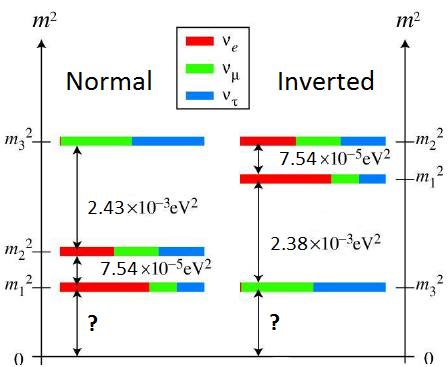
\includegraphics[width=.5\textwidth]{figures/hierarchy_alterred.png}
                \caption{The two possible hierarchies of neutrino masses.  The colors depict the mixing between the mass and flavor bases.}
\label{fig:numasshier}
\end{figure}

Neutrino oscillation demonstrates that neutrinos have non-zero mass, and though oscillation experiments measure the mass squared differences, the absolute masses of the three neutrinos remain unknown.  Cosmology puts limits on the sum of the three neutrino masses.  The Planck collaboration reports an upper bound on this sum at $\sum\limits_{i} m_{i} < 0.23$~eV \cite{Planck}.  The KATRIN experiment is expected to have a sensitivity of $m_{\bar{\nu}_{e}} < 0.2$~eV (90\% CL) for absolute neutrino mass from a careful measurement of tritium beta decay very near the maximal decay energy (Q-value) \cite{KATRIN}.

\section{Double Beta Decay}

Double beta decay is the simultaneous decay of two neutrons in a nucleus into two protons and two electrons.  It is observable in even-even nuclei only if beta decay is energetically forbidden or highly suppressed.  Two-neutrino double beta decay ($2\nu\beta\beta$), shown in Fig. \ref{fig:feynman_diags}(left), is allowed by the Standard Model and has been observed in about a dozen isotopes with half-lives around $10^{19}$-$10^{21}$ years.  Similar to beta decay, an anti-neutrino accompanies each electron in this decay, broadening the spectrum of the summed electron energy. This is a second-order process, and very rare, requiring low background to measure.

\begin{figure} %[H]
        %\centering
        %\begin{subfigure}
                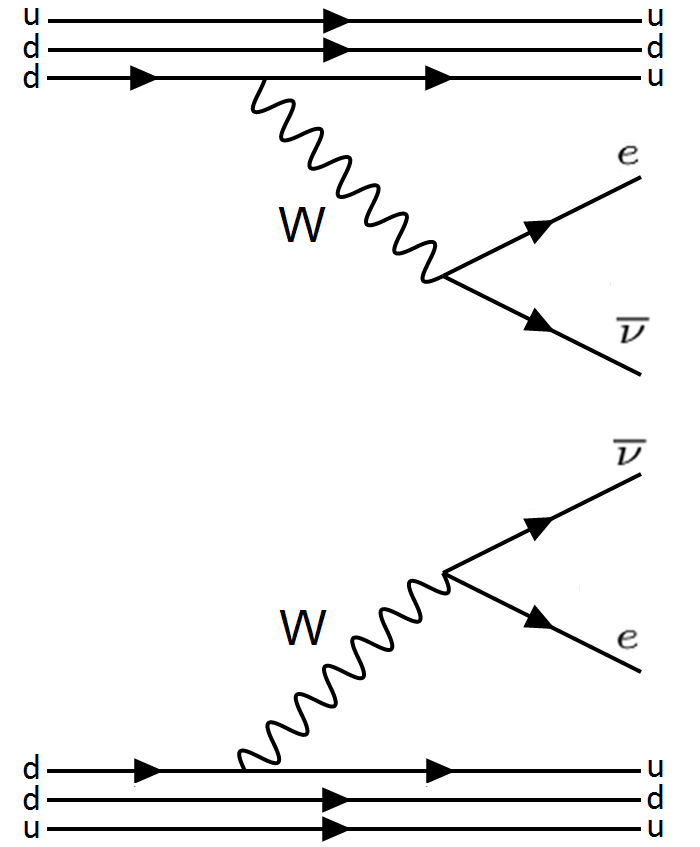
\includegraphics[width=.35\textwidth]{figures/feynman_2nu_quarks.png}
                %\caption{barf}
%        %\end{subfigure}
        %\begin{subfigure}
                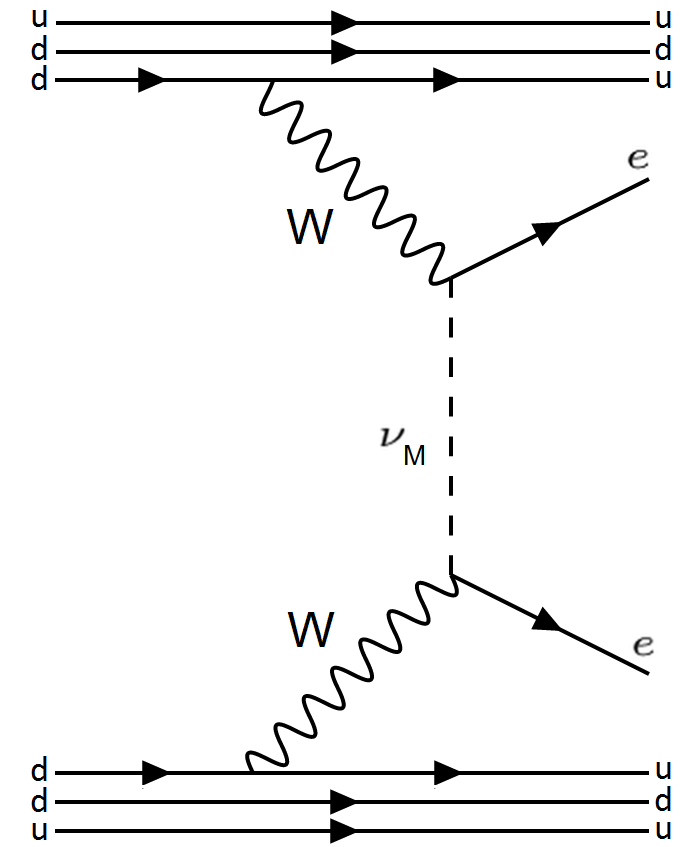
\includegraphics[width=.35\textwidth]{figures/feynman_0nu_quarks.png}
                \caption{Two-neutrino (left) and neutrinoless (right) double beta decay.}
        %\end{subfigure}
        \label{fig:feynman_diags}
\end{figure}

%\begin{table}[!htbp]
%\caption{$2\nu\beta\beta$ half-lives measured for various isotopes.} %not sure what [Small Table], between \caption and {}, w/ no spaces, does
%\label{table:bb_isotopes}
%\begin{tabular}{c|c|c}
%Isostope & $T^{2\nu}_{1/2} (10^{21}$~y) & Experiment\\
%\hline
%$^{136}$Xe & $2.165 \pm 0.016 \pm 0.059$ & EXO-200\\
%$^{76}$Ge & $1.84^{+0.14}_{-0.10}$ & GERDA\\
%\end{tabular}
%\end{table}

Neutrinoless double beta decay, shown in Fig. \ref{fig:feynman_diags}(right), is a postulated and yet unobserved mode of double beta decay. In this case, the neutrino is exchanged as a virtual particle (which would require that it is its own anti-particle, i.e. a Majorana particle), and there are no neutrinos in the final products. If discovered, neutrinos would be determined to be Majorana particles.  The decay would also demonstrate violation of lepton number conservation, as the final and initial states have lepton numbers of 2 and 0, respectively.  The measured $0\nu\beta\beta$ half-life would also aid in determining absolute neutrino mass according to Eq. \ref{eqn:rate_vs_mass}:

\begin{equation}
T_{1/2}^{0\nu} = (G^{0\nu}(Q,Z)|M^{0\nu}|^{2}\braket{m_{\nu}}^{2})^{-1}
\label{eqn:rate_vs_mass}
\end{equation}

\noindent
where $T_{1/2}^{0\nu}$ is the $0\nu\beta\beta$ half-life,  $G^{0\nu}$ is a known phase space factor, and $M^{0\nu}$ is a model-dependent nuclear matrix element.  $\braket{m_{\nu}}$ is the effective Majorana neutrino mass:

\begin{equation}
\braket{m_{\nu}} = \sum\limits_{i} U_{ei}^{2} m_{i}.
\label{eqn:effectivemass}
\end{equation}

\noindent
The terms $U_{ei}$ contain the measured mixing angles $\theta_{12}$ and $\theta_{13}$, as well as the unknown CP-violating phases $\delta$, $\alpha_1$, and $\alpha_2$.

The sum of the energies of the emitted electrons in double beta decay will serve as the distinction between the two-neutrino and zero-neutrino modes, shown in Fig. \ref{fig:spectrum_bb}. In the two-neutrino mode, the total decay energy is shared probabilistically between the electrons and the neutrinos (the nuclear recoil energy is negligible), resulting in a broad distribution in the summed electron energy. (Recall the similarly broad electron energy in single beta decay, which ultimately led to discovery of the neutrino involved.) But in the zero-neutrino mode, essentially all of the decay energy is carried away by the two electrons, resulting in effectively a single allowed value for the total electron energy -- a peak in the summed electron energy spectrum at the Q-value. 

\begin{figure} %[H]
        \centering
                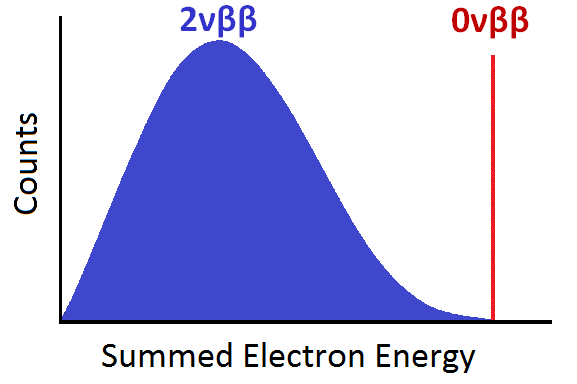
\includegraphics[width=.5\textwidth]{figures/spectrum_bb.png}
                \caption{Conceptual two-neutrino (blue) and zero-neutrino (red) double beta decay spectra.}
\label{fig:spectrum_bb}
\end{figure}

%  \emph{\color{red}make 0$\nu$ line shorter.}

The rarity of double beta decay requires very low backgrounds, especially around the Q-value for the $0\nu\beta\beta$ search. The next sections describe the experiments EXO-200 and its next-generation successor, nEXO, and how the barium tagging method studied in this work could be critical in obtaining essentially zero background in the second phase of nEXO operation.

\section{Enriched Xenon Observatory}

EXO-200 and nEXO (EXO standing for Enriched Xenon Observatory) are a progression of two experiments, each a liquid xenon (LXe) time projection chamber (TPC) designed to study the double beta decay of the isotope \textsuperscript{136}Xe, and ultimately to search for the zero-neutrino mode.  \textsuperscript{136}Xe is unique among the double beta decay isotopes in that it can be studied in a gas or liquid TPC instead of solid crystals, foils, or liquid scintillators.  The 3D event position reconstruction abilities of a TPC have advantages in background reduction, as described in section \ref{subsec:EXO200}.  Purification of Xe is straightforward and can be done continuously in the detector.  LXe is transparent, and produces substantial ionization and scintillation at 178~nm when energy is deposited in the LXe \cite{EXO200TwoNuLong}.  Xe is easy to isotopically enrich in centrifuges.  A liquid TPC approach also offers the opportunity to identify, or ``tag'', the daughter \textsuperscript{136}Ba\textsuperscript{++} ion at the site of the double beta decay event, which would provide a method for background-free identification of $0\nu\beta\beta$ \cite{Moe1991}. Barium tagging is the focus of our group at CSU and is the subject of this thesis.  The following sections decribe the EXO-200 experiment, as well as nEXO, the next-generation tonne-scale LXe TPC, which is now in the research and development stage.  EXO-200 does not have barium tagging implemented, but it is hoped that nEXO will incorporate barium tagging in the second phase of operation. 

\subsection{EXO-200}
\label{subsec:EXO200}

%\newline

Located about half a mile underground in the Waste Isolation Pilot Plant (WIPP) near Carlsbad, NM, EXO-200 has been operational since 2011.  It is a TPC containing around 170~kg of LXe enriched to 80.672 $\pm$ 0.14\% \textsuperscript{136}Xe \cite{EXO200TwoNuLong}. It is designed to probe Majorana neutrino masses down to around 100~meV \cite{EXO200instrumentationPart1}.  The WIPP mine is in a salt basin, which contains lower levels of Uranium and Thorium than rock in a typical mine.
%, with a fiducial volume corresponding to 66.20~kg of \textsuperscript{136}Xe

\begin{figure} %[H]
	\centering
	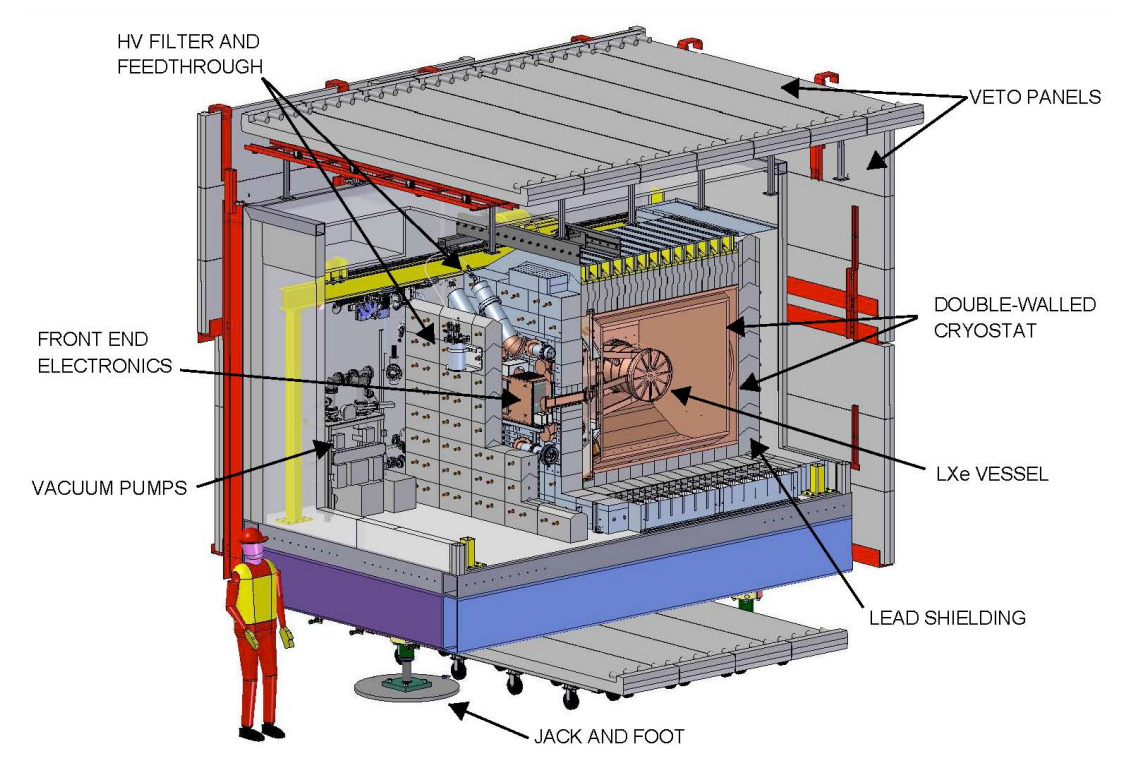
\includegraphics[width=.9\textwidth]{figures/cleanroom.png}
	\caption{Drawing of EXO-200 TPC Vessel with surrounding cryostat, lead walls, and muon veto panels.}
\label{fig:cleanroom}
\end{figure}

A schematic diagram of the TPC in the class 100 cleanroom is shown in Fig. \ref{fig:cleanroom}.  Several layers of lead wall surround the copper cryostat, which is filled with HFE-7000, a cryogenic fluid which keeps the TPC cooled to LXe temperatures  The HFE also provides shielding for the detector.  The TPC vessel is made of low-radioactivity copper, and is kept as thin as possible to minimize backgrounds.  Scintillating panels on the outside of the cleanroom provide a cosmic ray muon veto.

\begin{figure} %[H]
	\centering
	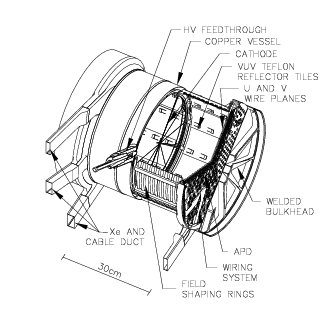
\includegraphics[width=.9\textwidth]{figures/TPC.png}
	\caption{EXO-200 TPC cutaway view \cite{EXO200TwoNuLong}.}
\label{fig:tpc}
\end{figure}

A cut-away view of the EXO-200 detector is shown in Fig. \ref{fig:tpc}.  It is two mirrored TPCs which share a cathode.  The detection planes are a combination of ionized charge induction/collection wires and large area avalanche photodiodes (LAAPDs), which detect scintillation light \cite{APDs}.

\begin{figure} %[H]
	\centering
	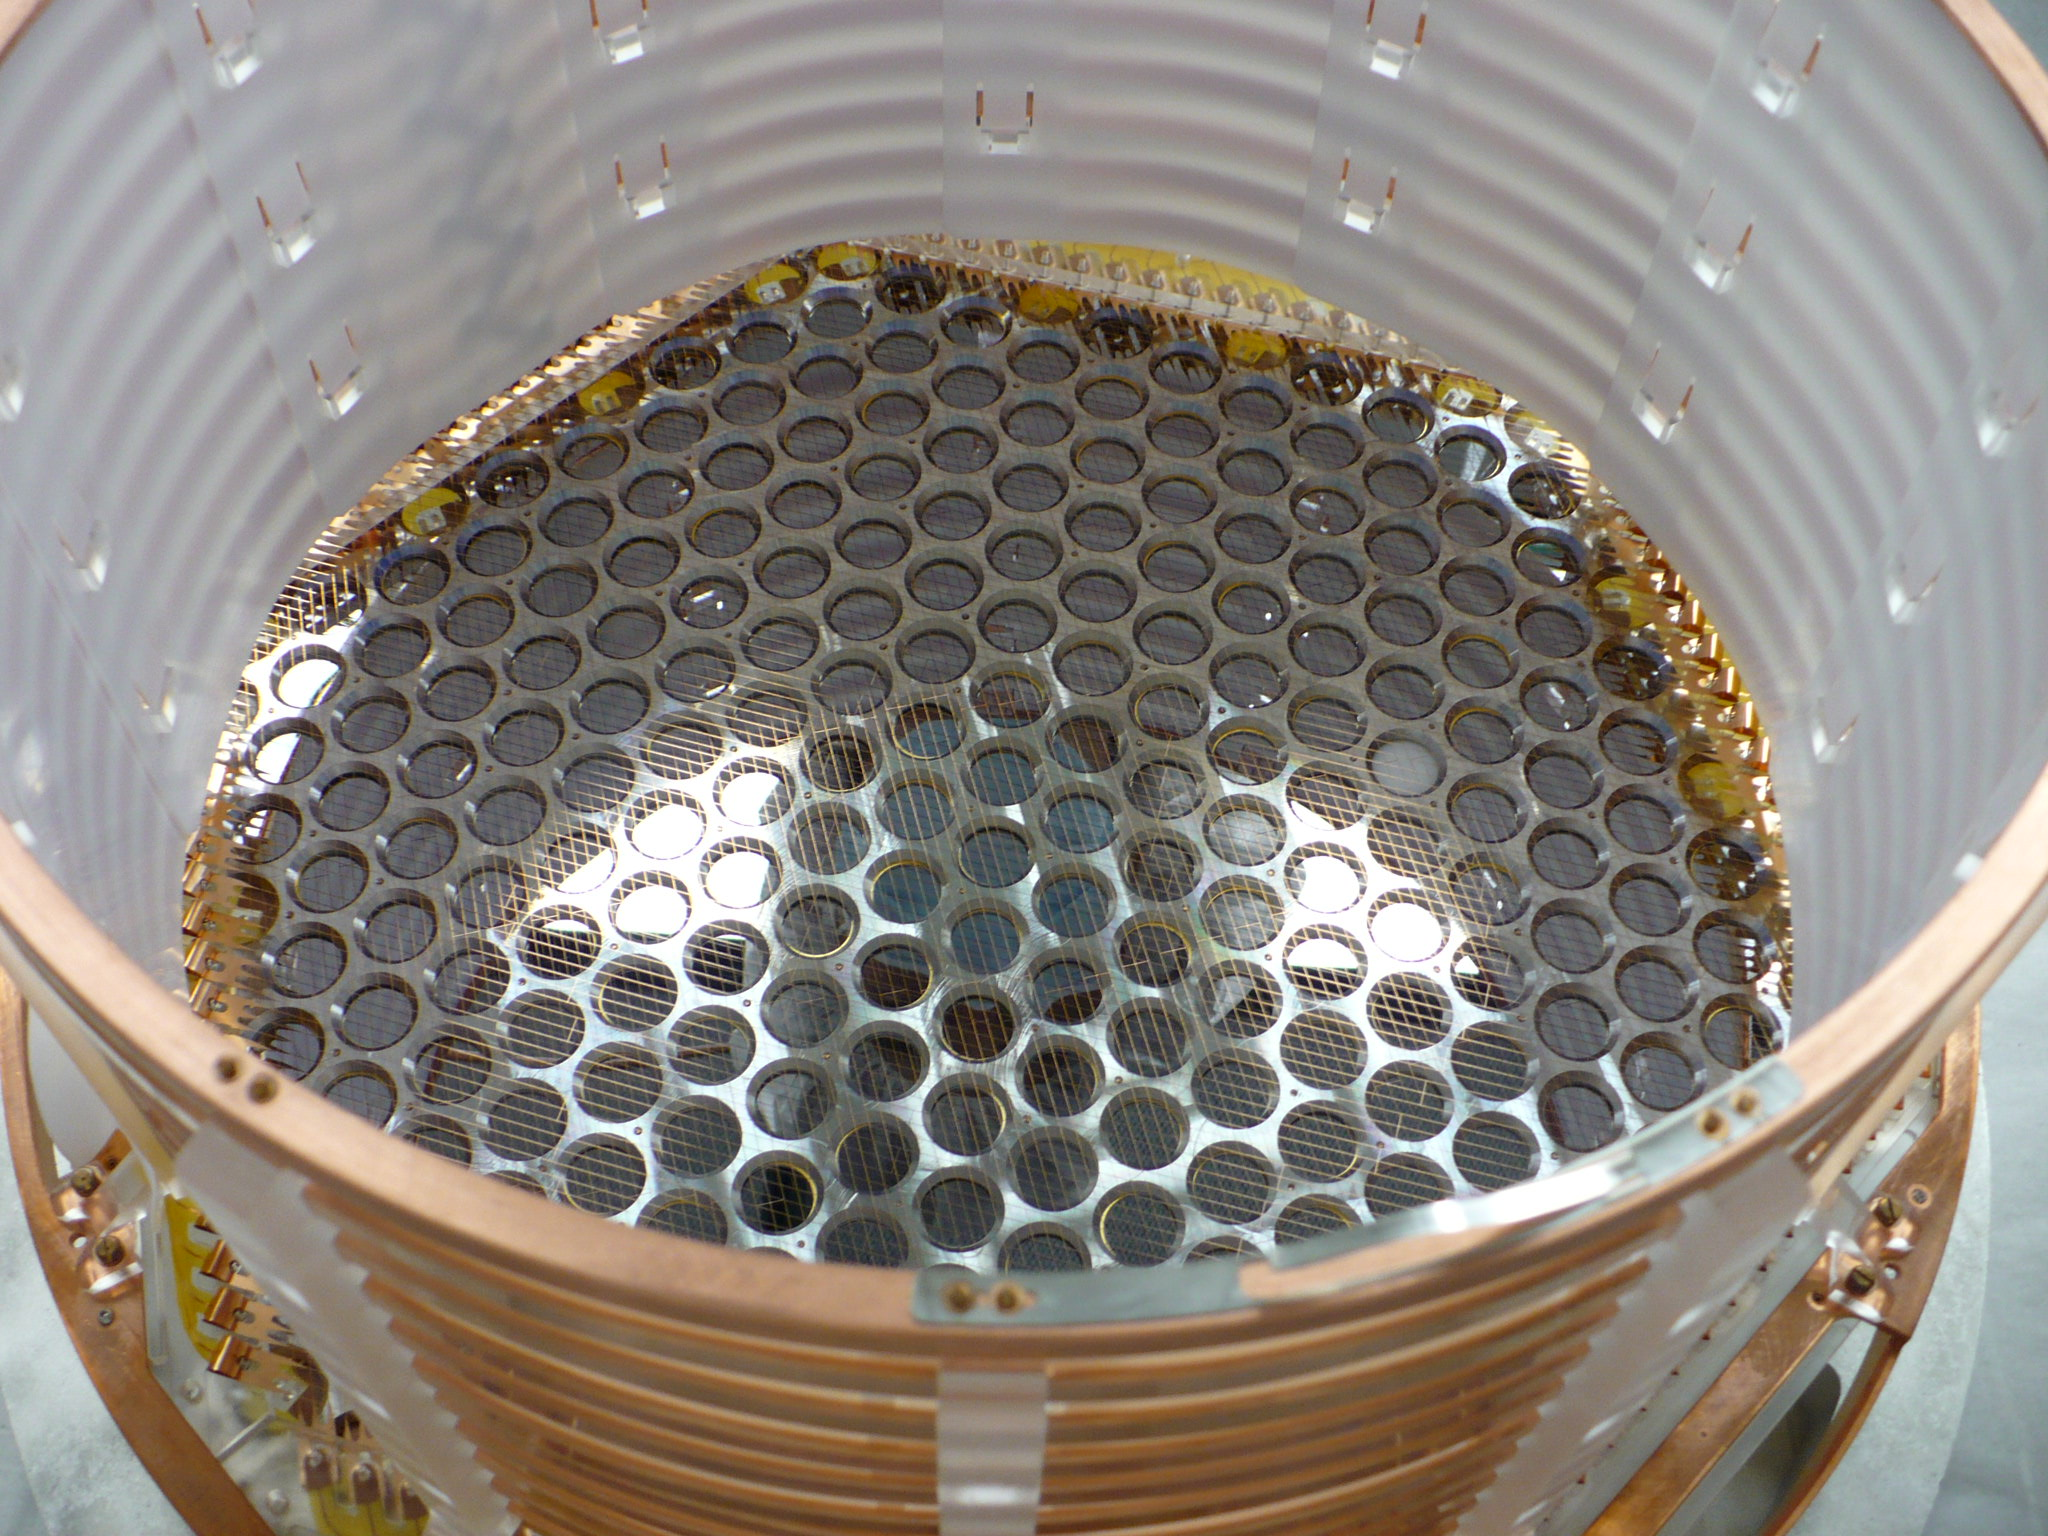
\includegraphics[width=.9\textwidth]{figures/TPCphoto.jpeg}
	\caption{View of the detection plane in one of the two EXO-200 TPCs.}
\label{fig:tpcphoto}
\end{figure}

A view into one of the TPCs is shown in Fig. \ref{fig:tpcphoto}.  On the detection plane, holes for the LAAPDs can be seen below the cross-hatched u- and v-wires.  The white material on the inner wall is the Teflon reflector.  When a double beta decay event occurs in the LXe, the energetic electrons ionize many surrounding Xe atoms, and also produce a scintillation signal.  %Scintillation light provides an initial time for z-measurement of the event, as well as an energy measurement.

\begin{figure} %[H]
	\centering
	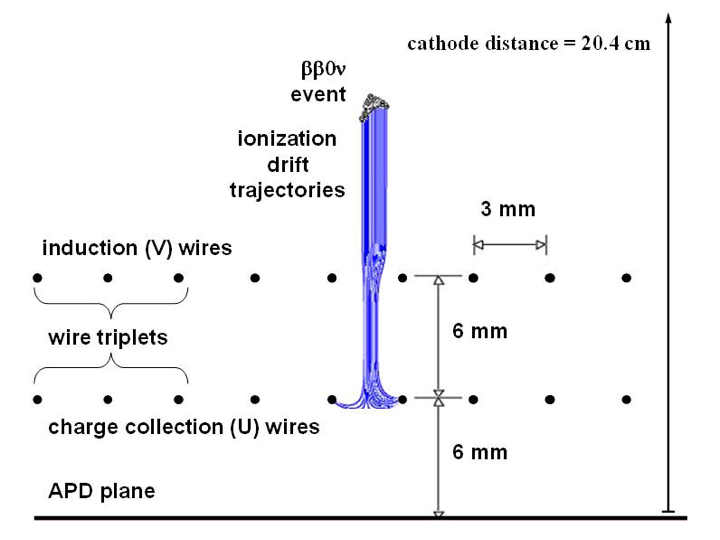
\includegraphics[width=.7\textwidth]{figures/anodecathodedriftcharges.png}
	\caption{EXO-200 event topology.  }
\label{fig:detectionplane}
\end{figure}

The cathode is set to -8~kV, providing an electric field of 374~V/cm across the 20~cm drift length of each TPC.  Ionized electrons drift from the decay site, first passing the v-wires, which receive an induction signal as depicted in Fig. \ref{fig:detectionplane}, and are then collected by the u-wires, which are set at a 60$^\circ$ angle from the v-wires.  An electric field of 778~V/cm between the u- and v-wires ensures 100\% v-wire transparency.  The charge collection provides an energy measurement.  Together, the u- and v-wires give an x/y position measurement for the event.  The time between the initial scintillation detection and the charge collection gives a z position.  Thus a 3D position can be reconstructed for the event if u-wire, v-wire, and scintillation signals are detected \cite{EXO200TwoNuLong}.

\begin{figure} %[H]
	\centering
	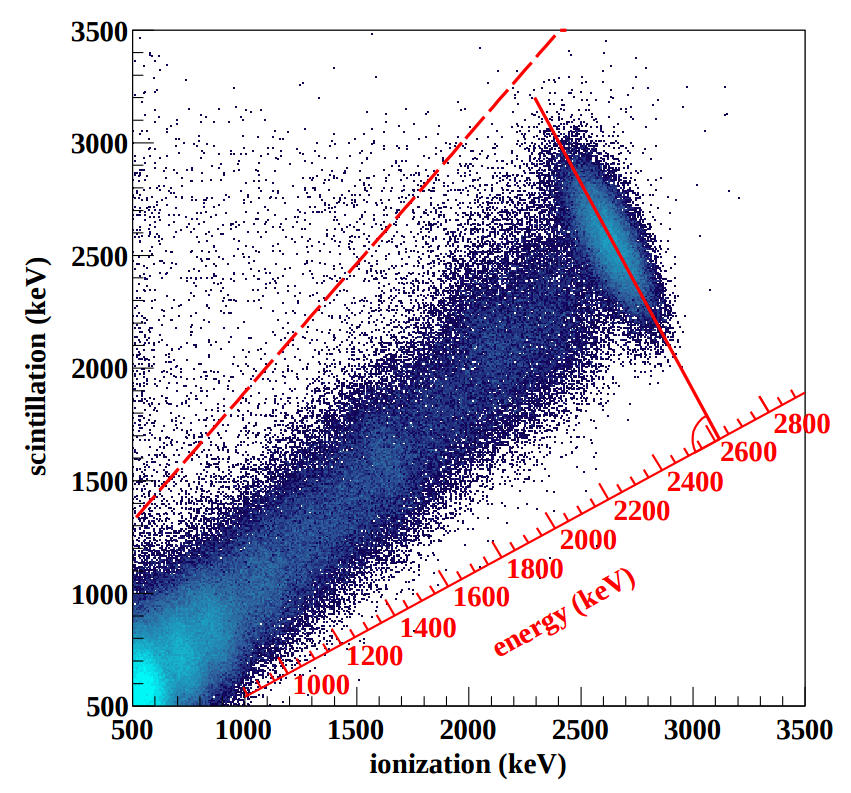
\includegraphics[width=.5\textwidth]{figures/anticorr.png}
	\caption{Anti-correlation between ionization and scintillation in events from the \textsuperscript{228}Th calibration source in EXO-200.  The dashed red line defines a cut on non-reconstructed events. \cite{EXO2000nuOriginal}}
\label{fig:antiCorr}
\end{figure}

Due to variable recombination of ionized electrons, ionization and scintillation signals of individual events in LXe are anti-correlated \cite{anticorr}.  This anti-correlation is exploited in EXO-200 to improve the energy resolution.  Energies measured by ionization and scintillation of events produced by the \textsuperscript{228}Th gamma source, one of the sources used to calibrate the EXO-200 detector, are plotted in Fig. \ref{fig:antiCorr}.  The tilt of the full absorption ellipse of the 2615~keV gamma line demonstrates the anti-correlation.  A ``rotated energy" is defined according to this tilt in order to optimize energy resolution.

%Energy resolution is important in a $0\nu\beta\beta$ search, as it distinguishes those events from $2\nu\beta\beta$ events in the tail of their spectrum.

Having a reconstructed 3D event position is important in several ways.  First, position-based corrections to scintillation and charge collection can be applied.  For charge, electronegative impurities in the LXe will absorb the drifting charge, requiring a drift-length (z-position) correction.  High purity levels, measured in terms of electron lifetime, of 2-5~ms and higher are maintained in EXO-200, resulting in a correction of a few percent for maximal drift lengths.  For scintillation, a 3D correction is applied, as some regions have more efficient light collection by the LAAPDs.  A 3D position also allows a fiducial volume to be defined.  A standoff distance from detector surfaces aids in distinction between gamma ray events and double beta decay events.  Gamma backgrounds, which mostly come from detector materials, exhibit some attenuation in the LXe volume.  Double beta decay events are uniformly distributed in the LXe.  Finally, 3D reconstruction allows the distinction between single-site (SS) and multi-site (MS) events.  A MS event is one where two spatially separated events occur in the same 2048-$\mu s$ time window.  These are mostly caused by gamma events, which can Compton-scatter one or more times in the LXe.  Rejecting MS events further aids in separating gamma events from double beta decay events \cite{EXO200TwoNuLong}.  Barium tagging will also benefit from a 3D reconstructed event position in nEXO.

%Calibration of EXO-200 is done using various radioactive sources which can be moved to several positions around the outside of the TPC.  Several different sources [\textsuperscript{137}Cs, \textsuperscript{60}Co, \textsuperscript{228}Th] span the energy range of interest, but the main source is $^{228}$Th, which produces gamma rays at [???]~MeV (\textsuperscript{208}Tl peak ... in chain right?), near the Q-value of $^{136}$Xe double beta decay where the $0\nu\beta\beta$ peak will be.  Source calibration data also provides a comparison between data and Monet-Carlo simulation, and provides the data for purity measurement and Light Map determination.  Data and Monte-Carlo for $^{228}$Th are shown in Fig. [ref fig source agreement].

\begin{figure} %[H]
	\centering
	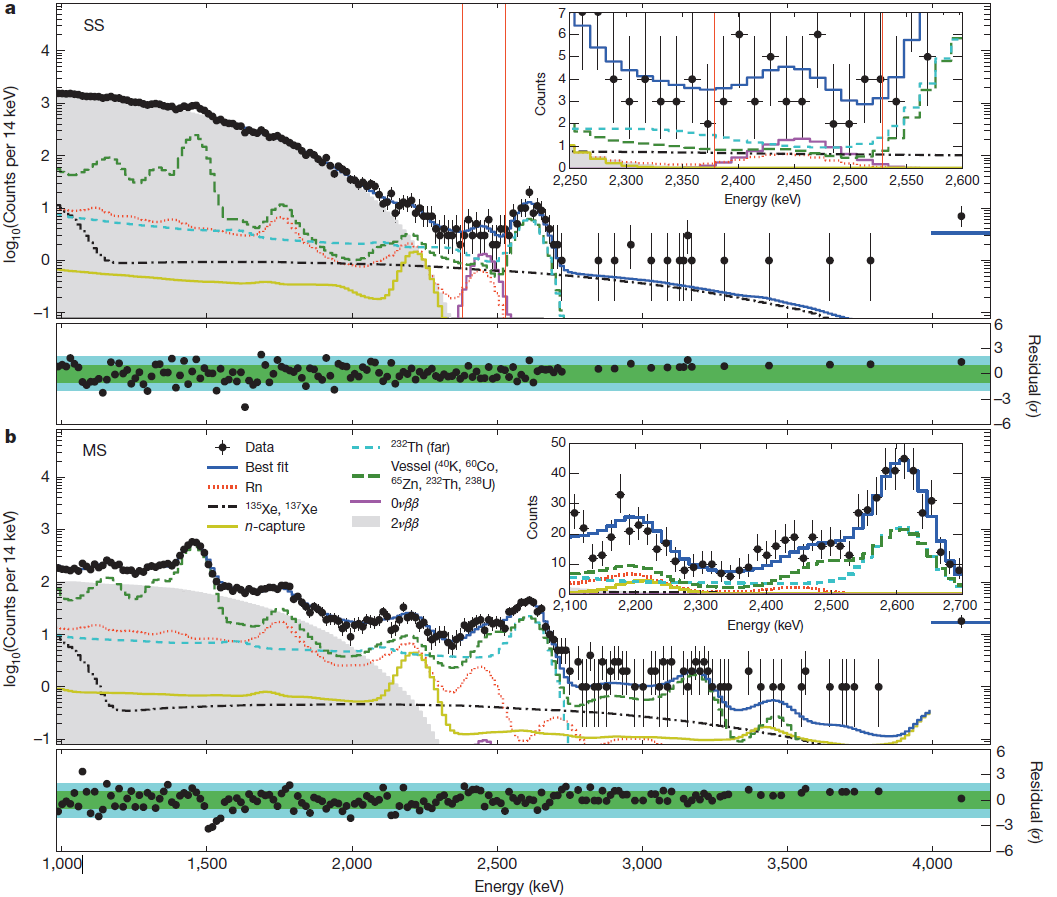
\includegraphics[width=.95\textwidth]{figures/0nu_spectrum_nature.png}
	\caption{EXO-200 energy spectrum of (a) single-site, and (b) multi-site events from the latest $0\nu\beta\beta$ search analysis.  The insets show a zoom into the region of interest around the $2\nu\beta\beta$ end point. \cite{EXO2000nuNature}}
\label{fig:exo200data}
\end{figure}

The final data set is fit using a combination of probability distribution functions (PDFs) for $0\nu\beta\beta$, $2\nu\beta\beta$, and background components.  Fits to the final energy spectrum data for (a)~SS events, and (b) MS events are shown in Fig. \ref{fig:exo200data} for the most recent $0\nu\beta\beta$ analysis.  The green bands beneath each plot show the residuals vs. energy.  The $2\nu\beta\beta$ spectrum, in gray, dominates the signal in the SS spectrum below the Q-value.  The vertical red lines in the SS spectrum outline the $\pm 2 \sigma$ region of interest around the Q-value, where the $0\nu\beta\beta$ peak will lie.  The insets are a zoom into this region.  The best fit value for $0\nu\beta\beta$ in this dataset is non-zero, but it is consistent with the null hypothesis at $1.2 \sigma$.  This sets an upper limit on the $0\nu\beta\beta$ half-life at $T^{0\nu\beta\beta}_{1/2} < 1.1 \times 10^{25}$~yr (90\% CL), which corresponds to $\braket{m_{\nu_{e}}} < $190-450~meV depending on nuclear matrix element calculations \cite{EXO2000nuNature}.  The $2\nu\beta\beta$ half-life has also been measured in EXO-200 as $T^{2\nu\beta\beta}_{1/2} = 2.165 \pm 0.016$(stat)$ \pm 0.059$(sys)$ \times 10^{21}$~yr \cite{EXO200TwoNuLong}.  This is the most precise $2\nu\beta\beta$ measurement to date and is consistent with previous measurements by EXO-200 in 2011 \cite{EXO200TwoNuOriginal} and KamLAND-ZEN in 2012 \cite{KamLAND}.

\subsection{nEXO}

The next-generation successor to EXO-200 is nEXO, a $\sim$5~ton LXe TPC which will probe Majorana neutrino masses down to the 10~meV scale.  A schematic diagram of the nEXO detector in the SNOLAB cryopit, one of the possible locations for nEXO, is shown in Fig. \ref{fig:nEXO_cryopit}.  Similar to EXO-200, the copper-housed TPC will be submerged in HFE fluid, inside a copper cryostat.  The cryostat will be insulated and submerged in a large volume of water shielding, in which photo-multiplier tubes will provide a muon veto by observing Cherenkov radiation.  nEXO will be a single TPC.  Rather than wires, nEXO will use tile electrodes for charge readout, shown in Fig. \ref{fig:nEXO_readout}.  Silicon photo-multipliers on the sides of the detector will be used for light detection.

\begin{figure} %[H]
	\centering
	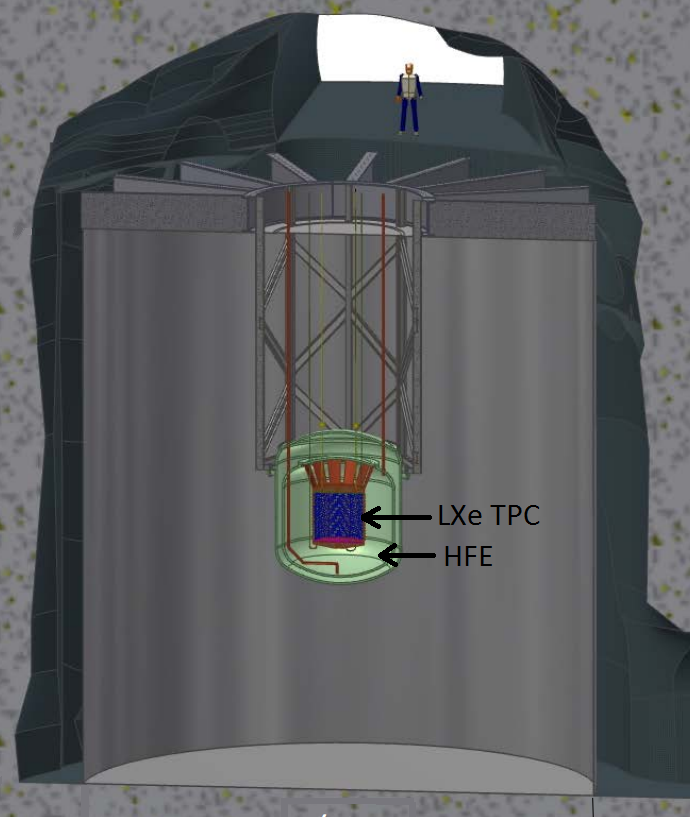
\includegraphics[width=.7\textwidth]{figures/nEXO_cryopit.png}
	\caption{nEXO TPC in the SNOLAB cryopit.}
\label{fig:nEXO_cryopit}
\end{figure}

\begin{figure} %[H]
	\centering
	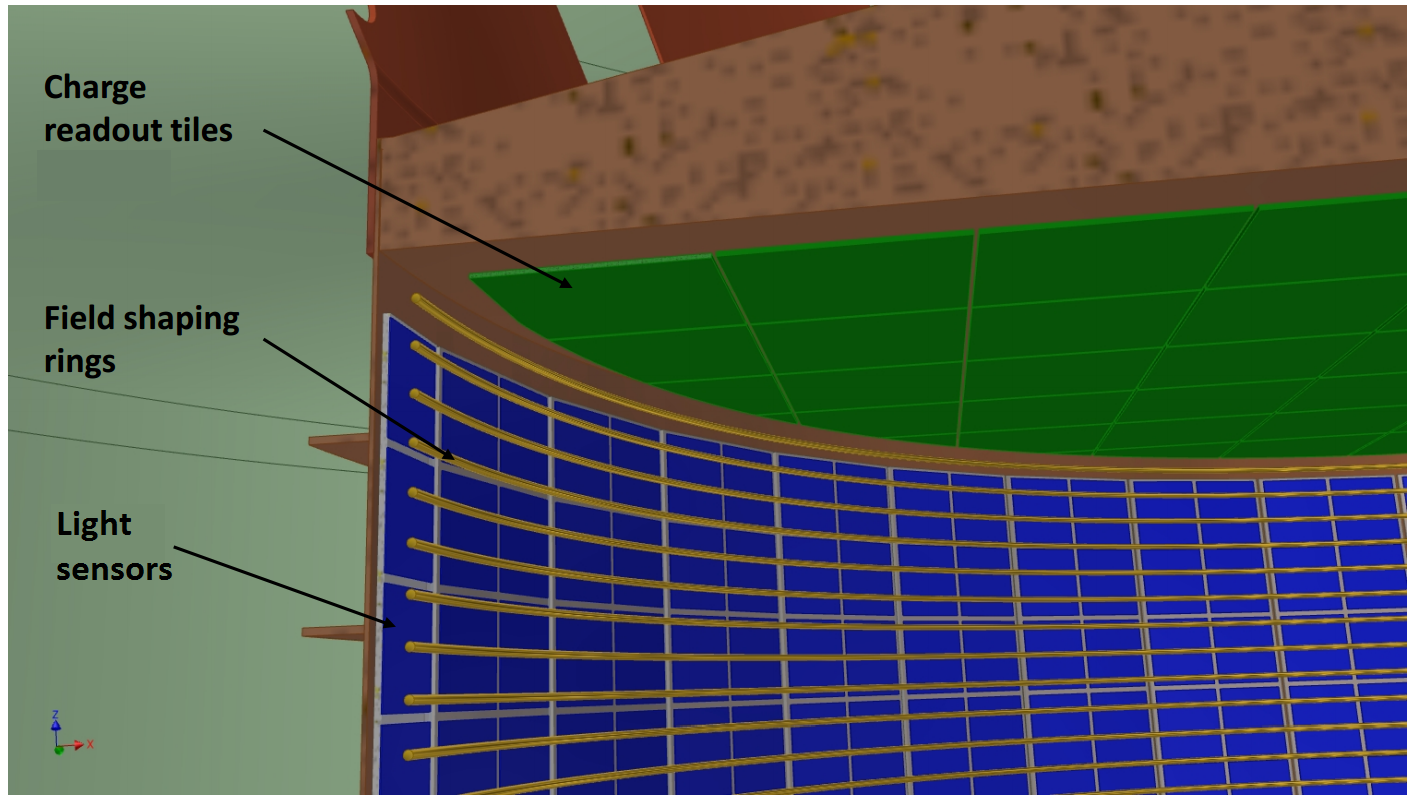
\includegraphics[width=.7\textwidth]{figures/nEXO_readout.png}
	\caption{nEXO readout.}
\label{fig:nEXO_readout}
\end{figure}

The sensitivity projections for nEXO are shown in Fig. \ref{fig:sensitivity_nEXO}, along with those of EXO-200.  EXO-200 probes the degenerate mass region down to about 0.1~eV.  nEXO will reach the non-degenerate region where the two possible mass hierarchies split, and will probe the full inverted hierarchy.  The addition of barium tagging would be a very significant advance, as it would push the mass sensitivity down into the region allowed only by the normal hierarchy.

% {\color{gray}[ref for this?]}

\begin{figure} %[H]
	\centering
	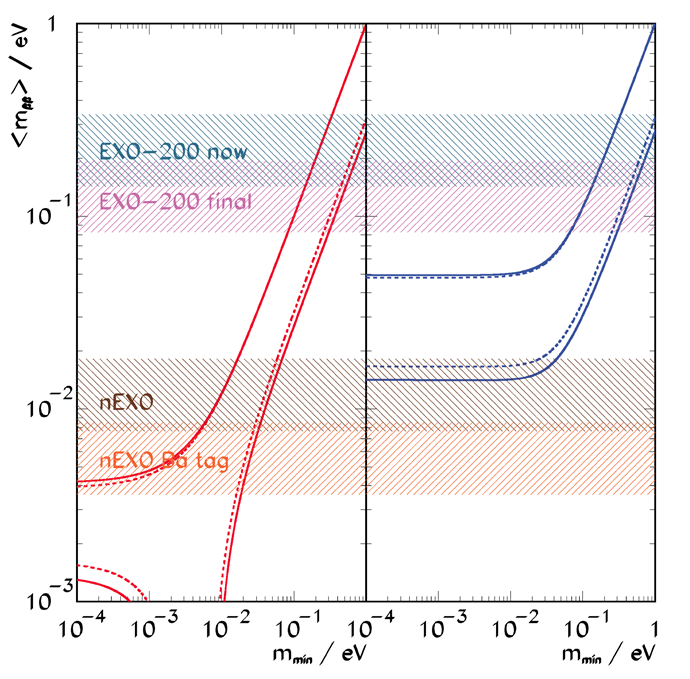
\includegraphics[width=.7\textwidth]{figures/sensitivity_v2.png}
	\caption{nEXO projected sensitivity to the effective Majorana neutrino mass vs. the minimum of the three masses neutrino m$_{min}$.  The dotted (solid) lines denote the 1(2)-$\sigma$ region allowed by neutrino oscillation measurements.}
\label{fig:sensitivity_nEXO}
\end{figure}

\subsection{Barium Tagging}

The ability to observe the daughter of each $0\nu\beta\beta$ event is the ultimate background rejection technique.  No background events generate a Ba daughter except $2\nu\beta\beta$ of \textsuperscript{136}Xe \cite{Moe1991}.  Several possible barium tagging techniques have been proposed for nEXO.  The original and most natural concept is to direct one or more lasers at the decay site to induce fluorescence of the barium daughter.  This technique was explored by our group, and has been abandoned for now because Ba\textsuperscript{+} fluorescence was not unambiguously identified in LXe \cite{Kendy}.

%Another concept was to grab the daughter in SXe on a cold probe, similar to the method explored in this thesis, but to then evaporate the SXe and drift the daughter into a trap for detection in vacuum.  This method was abandoned when extraction of barium from SXe samples could not be achieved by Liang Yang's group [ref?].

A few barium tagging techniques continue to be explored.  One of these is to grab the daughter on a probe surface, brought to the decay site by a probe.  It would then be moved to a location where it can be desorbed from that surface by an infrared laser, and subsequently resonantly ionized by two lasers in order to detect it by time-of-flight spectroscopy.  The apparatus for the study of this method is described in \cite{Twelker2014}, along with some initial results.

The other leading technique for barium tagging in LXe, now the focus of our group and the subject of this thesis, is barium tagging in solid xenon (SXe).  In this method, a cold probe would be inserted to the site of the candidate $0\nu\beta\beta$ event, and additional cooling would be applied to trap the Ba or Ba\textsuperscript{+} daughter in a small amount of SXe.  The single Ba/Ba\textsuperscript{+} would be observed by laser-induced fluorescence in the SXe, a technique more generally called matrix isolation spectroscopy.  A concept for a probe is shown in Fig. \ref{fig:probe}.  The SXe layer is formed on a sapphire window at the end of the probe.  Sapphire is a good candidate for a substrate because it has good thermal conductivity at low temperature and is highly transparent.  An excitation laser may be brought into the probe through a fiber, and scanned across the sapphire to excite the Ba/Ba\textsuperscript{+} in the SXe.  A return fiber could collect the laser reflection to measure the SXe thickness via interference fringes.  The Ba/Ba\textsuperscript{+} fluorescence would then be collected by a lens/filter system and imaged onto a CCD.  Additional components, not shown, would be required for cooling the sapphire, either by liquid He or by a Joule-Thompson nozzle.

\begin{figure} %[H]
	\centering
	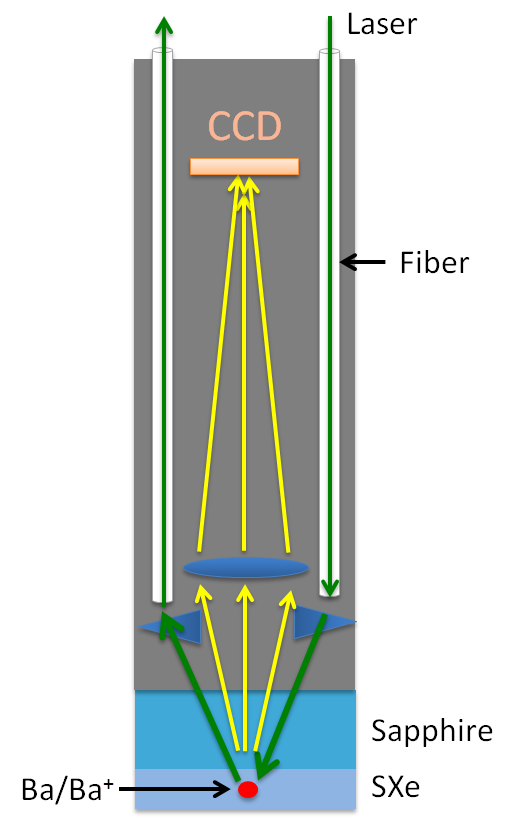
\includegraphics[width=.5\textwidth]{figures/probe_flat.png}
	\caption{Concept for a cryoprobe for \textsuperscript{136}Ba\textsuperscript{+} daughter ion capture and detection in SXe, and a concept for internal collection optics.}
\label{fig:probe}
\end{figure}

Whether the daughter Ba will neutralize or remain ionized in SXe is not yet known.  It is expected that a Ba\textsuperscript{++} daughter of $0\nu\beta\beta$ will neutralize rapidly to Ba\textsuperscript{+} by charge transfer in LXe, since the LXe conduction band gap is slightly less than the ionization potential for Ba\textsuperscript{+} \cite{Moe1991}.  Further neutralization by recombination with the electron cloud could also occur.  However, a study of neutralization of \textsuperscript{214}Bi daughters of \textsuperscript{214}Pb beta decay in EXO-200 has observed a high percentage, 76(5)\%, of ionized daughters, and negligible subsequent neutralization in many minutes \cite{alphaion}.  This provides an expectation of a high percentage of ionized \textsuperscript{136}Ba daughters of $0\nu\beta\beta$ in LXe in the singly ionized state.

%The next chapter describes theory relevant to single Ba/Ba\textsuperscript{+} detection in SXe matrices.